% Created 2017-01-10 Tue 16:02
% Intended LaTeX compiler: pdflatex
\documentclass[presentation, bigger]{beamer}
\usepackage[no-math]{fontspec}
\usepackage[BoldFont,SlantFont,AutoFakeBold=true,AutoFakeSlant=true]{xeCJK}
\setCJKmainfont[BoldFont=FandolSong-Bold.otf,ItalicFont=FandolKai-Regular.otf]{FandolSong-Regular.otf}
\setCJKsansfont[BoldFont=FandolHei-Bold.otf]{FandolHei-Regular.otf}
\setCJKmonofont{FandolFang-Regular.otf}
\usefonttheme[stillsansseriflarge,stillsansserifsmall]{serif}
\usepackage{graphicx}
\usepackage{xcolor}
\usepackage{listings}
\defaultfontfeatures{Mapping=tex-text}
\usepackage{geometry}
\usepackage{verbatim}
\usepackage{fixltx2e}
\usepackage{longtable}
\usepackage{float}
\usepackage{wrapfig}
\usepackage{rotating}
\usepackage[normalem]{ulem}
\usepackage{amsmath}
\usepackage{marvosym}
\usepackage{wasysym}
\usepackage{amssymb}
\usepackage{hyperref}
\setlength{\parindent}{0in}
\tolerance=1000
\usetheme{metropolis}
\author{刘恩泽}
\date{2017-01-03}
\title{品类分析}
\hypersetup{
 pdfauthor={刘恩泽},
 pdftitle={品类分析},
 pdfkeywords={},
 pdfsubject={},
 pdfcreator={Emacs 25.1.1 (Org mode 9.0.3)},
 pdflang={English}}
\begin{document}

\maketitle
\begin{frame}{目录}
\tableofcontents
\end{frame}

\section{整体数据}
\label{sec:org2a13ad8}
\begin{frame}[label={sec:orged2f9cc}]{购买时间分布}
\begin{center}
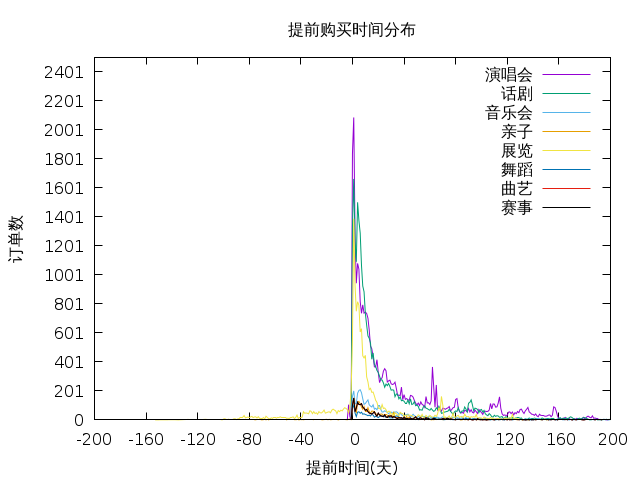
\includegraphics[width=.9\linewidth]{./image/time-distribution.png}
\end{center}
\end{frame}

\begin{frame}[label={sec:orge518a8b}]{溢价比例分布}
\begin{center}
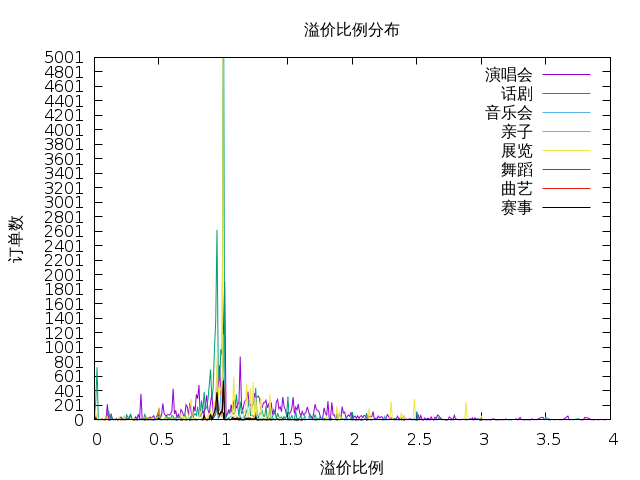
\includegraphics[width=.9\linewidth]{./image/over-distribution.png}
\end{center}
\end{frame}
\begin{frame}[label={sec:org855a38b}]{注册购买时间分布}
\begin{center}
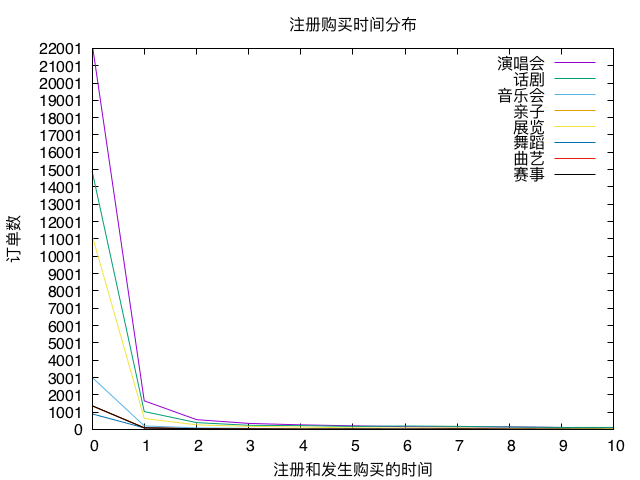
\includegraphics[width=.9\linewidth]{./image/register-distribution.png}
\end{center}
\end{frame}

\begin{frame}[label={sec:orgf7ebcbb}]{成交价格分布}
\begin{center}
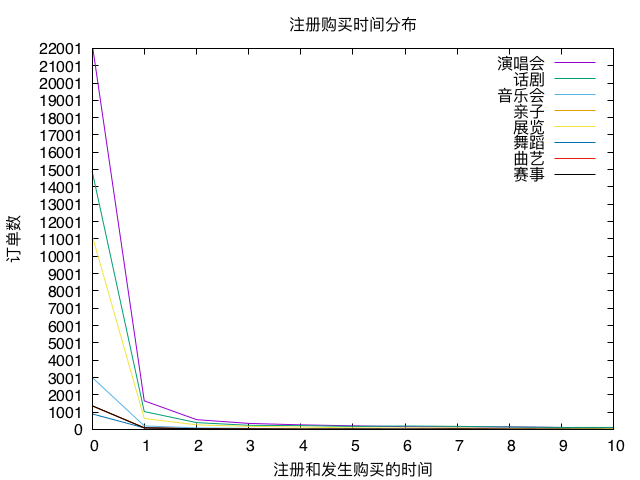
\includegraphics[width=.9\linewidth]{./image/register-distribution.png}
\end{center}
\end{frame}

\begin{frame}[label={sec:org6fb88ae}]{决策时间分布}
\begin{center}
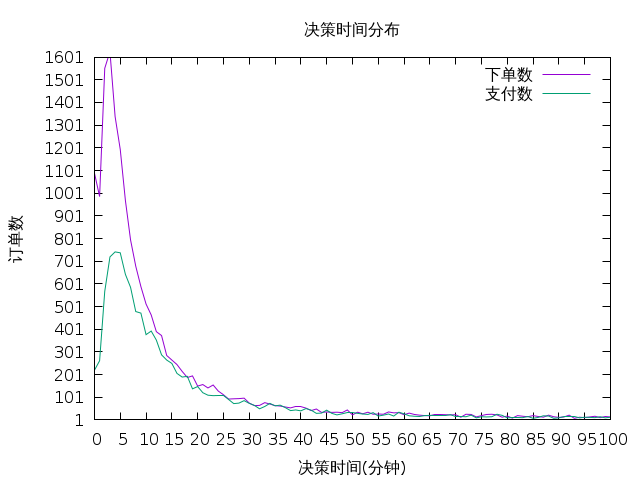
\includegraphics[width=.9\linewidth]{./image/decision-distribution.png}
\end{center}
\end{frame}

\section{APP 行为数据}
\label{sec:org43fa7c8}
\begin{frame}[label={sec:org9b565fe}]{访问量 TOP 的页面}
百分比表示占整体流量的多少
\begin{enumerate}
\item 演出详情页 20\%
\item 首页 18.9\%
\item 列表页 12.8\%
\item 选票页 11.3\%
\item 个人中心 5.8\%
\item 订单列表 3\%
\item 订单详情 3\%
\item 确认订单页 2.6\%
\end{enumerate}
\end{frame}

\begin{frame}[allowframebreaks,label=]{主要页面转化}
\begin{itemize}
\item 演出详情页
\begin{description}
\item[{3.4\%}] exit
\item[{30\%}] 选票页
\item[{20\%}] 列表页
\item[{7.8\%}] 首页
\item[{7.2\%}] 演出详情(相关演出)
\end{description}
\item 首页
\begin{description}
\item[{12.3\%}] exit
\item[{34\%}] 列表页
\item[{17.7\%}] 个人中心
\item[{9.4\%}] 演出详情
\end{description}
\end{itemize}
\framebreak
\begin{itemize}
\item 列表页
\begin{description}
\item[{7\%}] exit
\item[{47.7\%}] 演出详情
\item[{21.4\%}] 首页
\item[{10\%}] 选票页(购买)
\item[{8.9\%}] 列表页(继续搜索)
\end{description}
\item 选票页
\begin{description}
\item[{10\%}] exit
\item[{48.3\%}] 演出详情
\item[{12.3\%}] 下单页
\item[{11.8\%}] 选票页(换票档选择?)
\end{description}
\end{itemize}
\end{frame}

\section{演唱会}
\label{sec:org31909c0}
\begin{frame}[allowframebreaks,label=]{订单分布}
演唱会总订单 31000+, 前 10 的演出订单 11215. 有订单演出共 647 个. 小于 10 单的演出 300+.
\begin{center}
\begin{tabular}{lr}
演出名称 & 订单数\\
\hline
五月天 上海站 & 2370\\
学友.经典 上海站 & 1653\\
2016 上海简单生活节 & 1463\\
2016 五月天 北京站 & 1214\\
陈奕迅 -北京鸟巢站 & 1114\\
学友.经典 北京站 & 895\\
中国新歌声总决赛暨巅峰之夜 & 737\\
上海滴水湖春浪音乐节 & 616\\
学友.经典 广州站 & 595\\
张杰 2016“我想”北京站 & 558\\
\end{tabular}
\end{center}

\framebreak
排名前 50 的演出订单量 21285 万, 涉及的关键词为:

\begin{quote}
五月天;张学友;上海简单生活节;陈奕迅;中国新歌声;
春浪音乐节;张杰;长阳音乐节;周杰伦;陈慧娴;陈奕迅;
BIGBANG;草莓音乐节;好妹妹乐队;
热波音乐节;罗大佑;崔健;刘若英;
李荣浩;风暴电音节;张信哲;宋仲基;蔡健雅;田馥甄;
张惠妹;梁静茹;林忆莲;马克西姆
\end{quote}
\end{frame}

\begin{frame}[allowframebreaks,label=]{点击分布}
演唱会总点击 560 万, 前 10 的演出点击 165 万, 前 10 的演出除了五月天,其他转化率在千 2 和千 9 之间
\begin{center}
\begin{tabular}{lrrr}
演出名称 & 订单数 & 点击数 & 转化率\\
\hline
学友.经典 上海站 & 1653 & 256915 & 0.0064\\
2016 周杰伦 上海站 & 517 & 225648 & 0.0023\\
2016 周杰伦 北京站 & 345 & 216424 & 0.0016\\
2016 五月天 上海站 & 2370 & 189998 & 0.0125\\
2016 BIGBANG SHANGHAI & 375 & 176637 & 0.0021\\
陈奕迅 北京鸟巢站 & 1114 & 165120 & 0.0067\\
陈奕迅 上海站 & 407 & 116387 & 0.0035\\
学友.经典 广州站 & 595 & 112771 & 0.0053\\
学友.经典 北京站 & 895 & 99861 & 0.009\\
2016 五月天 北京站 & 1214 & 95994 & 0.0126\\
\end{tabular}
\end{center}

\framebreak
排名前 50 的演出点击量为 350 万, 涉及的关键词为:

\begin{quote}
张学友;周杰伦;五月天;BIGBANG;陈奕迅;宋仲基;王菲;
刘若英;中国新歌声;简单生活节;SNH48;张杰;
echo;回声嘉年华音乐节; 蔡依林;张信哲;
张惠妹;长阳音乐节;百威风暴电音节;
陈慧娴;浙江卫视;湖南卫视;田馥甄;
\end{quote}
\end{frame}

\begin{frame}[label={sec:org543807a}]{转化率分布}
\begin{description}
\item[{转化率最高: 17\%}] 130*90 铝膜双面加厚 音乐节防潮垫 票牛特价
\item[{转化率最低: 0.04\%}] SNH48
\item[{转化率 1\% 以上的 83 个}] 总点击 77 万, 总成单 12353, 客单均价 300-400 左右
\end{description}
\end{frame}
\begin{frame}[label={sec:org93b5adb}]{交易额分布}
总交易额 4344 万, 前 10 的演出 2000 万, 前 20 的演出 2560 万, 前 10 的客单均价在 2000-3000 左右

交易额前 10 的演出为:
\begin{center}
\begin{tabular}{lrrrr}
演出名称 & 订单量 & 点击数 & 转化率 & 总流水\\
\hline
学友.经典 上海站 & 1653 & 256915 & 0.0064 & 5400668\\
五月天 上海站 & 2370 & 189998 & 0.0125 & 3265187\\
学友.经典 北京站 & 895 & 99861 & 0.009 & 2207305\\
周杰伦 上海站 & 517 & 225648 & 0.0023 & 1853747\\
陈奕迅 北京鸟巢站 & 1114 & 165120 & 0.0067 & 1600086\\
学友.经典 广州站 & 595 & 112771 & 0.0053 & 1586930\\
BIGBANG  SHANGHAI & 375 & 176637 & 0.0021 & 1328730\\
五月天 北京站 & 1214 & 95994 & 0.0126 & 1256848\\
周杰伦 北京站 & 345 & 216424 & 0.0016 & 1239325\\
\end{tabular}
\end{center}
\end{frame}

\begin{frame}[label={sec:org57a064d}]{价格分布}
\begin{center}
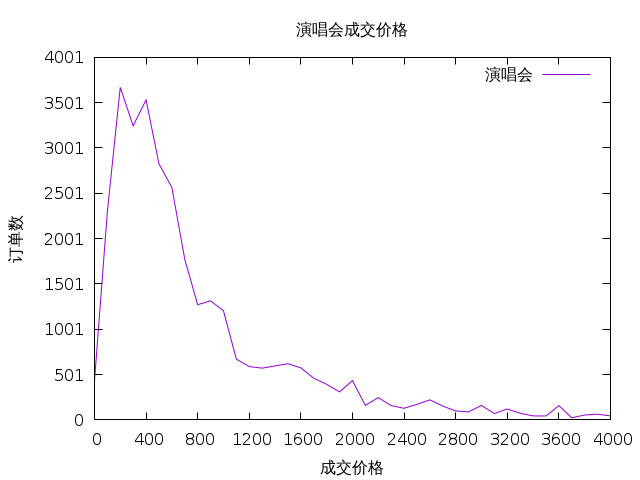
\includegraphics[width=.9\linewidth]{./image/vocal-price-distribution.png}
\end{center}
\end{frame}

\begin{frame}[label={sec:org1c1c11e}]{订单票数分布}
\begin{center}
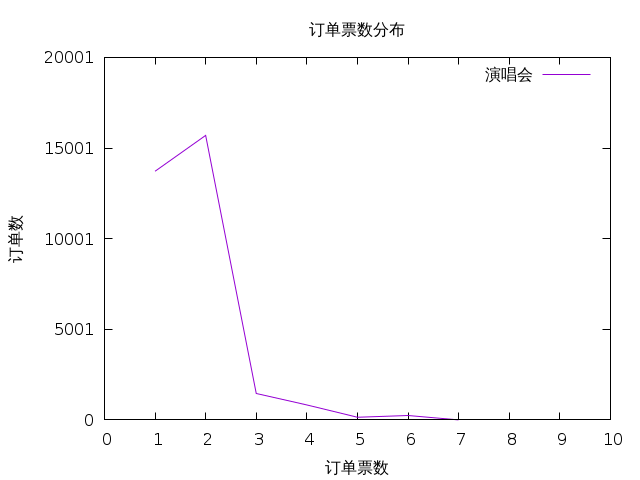
\includegraphics[width=.9\linewidth]{./image/order-tickets-distribution.png}
\end{center}
\end{frame}

\begin{frame}[label={sec:org3a43e9f}]{行为路径分析}
\alert{没做出来,未完待续\ldots{}}
\end{frame}
\begin{frame}[label={sec:orgead1a8a}]{购买用户分析}
\begin{itemize}
\item 演唱会购买用户共 26800 人
\item 2800 个演唱会购买用户会买其他类目
\item 5800 个演唱会用户有复购行为
\begin{center}
\begin{tabular}{rr}
购买单数 & 用户数\\
\hline
1 & 21520\\
2 & 3163\\
3 & 920\\
4 & 417\\
5 & 196\\
6 & 136\\
7 & 78\\
8 & 61\\
\end{tabular}
\end{center}
\end{itemize}
\end{frame}

\section{话剧}
\label{sec:org317ff9c}
\begin{frame}[allowframebreaks,label=]{订单分布}
\begin{quote}
有一定的品牌效应, 但整体话剧分布更均匀, 长尾效应也更明显
\end{quote}
\begin{itemize}
\item 话剧总订单 28585
\item 前 10 的话剧订单 6000
\item 超过 100 单的话剧共 60 个
\item 小于 10 单的话剧共 655 个
\item 有订单的话剧共 1040 个
\item 不眠之夜订单 1114
\item 恋爱的犀牛订单 897
\end{itemize}
\end{frame}

\begin{frame}[allowframebreaks,label=]{点击分布}
\begin{quote}
从这个维度没看出啥特别的,整体很平滑
\end{quote}
\begin{itemize}
\item 点击最高的如梦之梦和不眠之夜,点击数基本一样,5 万多
\item 点击数上万的 42 个
\item 点击数上千的 352 个
\item 点击数上百的 621 个
\item 点击数小于 100 的 25 个
\end{itemize}
\end{frame}

\begin{frame}[label={sec:org3eb3c5c}]{转化率分布}
转化率超过 10\%的 13 个演出 (猜和早期量少关系很大)
\begin{itemize}
\item 契诃夫名剧《万尼亚舅舅》 3.1565
\item 开心麻花爆笑舞台剧《小丑爱美丽》2.76
\item 话剧《恋爱的犀牛》 1.16
\item 开心麻花 2016 爆笑舞台剧《李茶的姑妈》 0.82
\item 开心麻花爆笑舞台剧《乌龙山伯爵》 0.5204
\item 孟京辉戏剧作品《希特勒的肚子》 0.4271
\item 开心麻花爆笑舞台剧《江湖学院》 0.3284
\item 韩国第一音乐喜剧《乱打神厨》 0.2274
\item 歌剧《一江春水向东流》音乐会版 0.1667
\item 开心麻花爆笑舞台剧《羞羞的铁拳》 0.1515
\item 繁星戏剧 都市爱情喜剧《那次奋不顾身的爱情》 0.1273
\item 百老汇音乐剧《我,堂吉诃德》中文版 0.1077
\end{itemize}
\end{frame}

\begin{frame}[label={sec:org9b28387}]{交易额分布}
总交易额 1289 万, 前 10 的销售 481 万.
\begin{itemize}
\item 不眠之夜 117 万
\item 如梦之梦 114 万
\item 舞马 53 万
\item 乌龙山伯爵 31 万
\item 恋爱的犀牛 27 万
\item 三体 22 万
\item 戏台 19 万
\item 无人生还 18 万
\item 莫扎特 18 万
\end{itemize}
\end{frame}
\begin{frame}[label={sec:orgc2051d9}]{价格分布}
\begin{center}
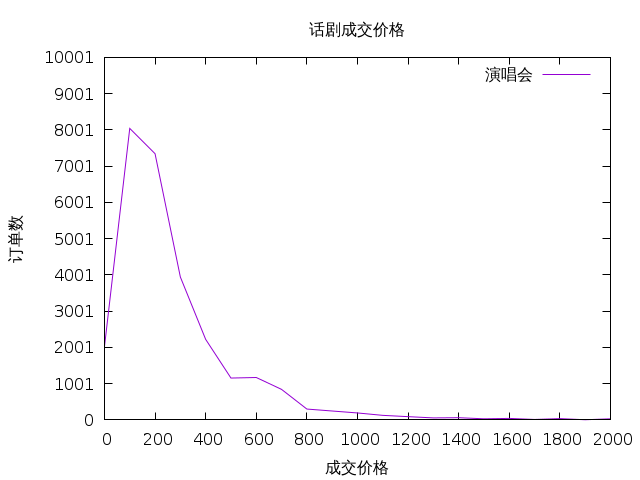
\includegraphics[width=.9\linewidth]{./image/drama-price-distribution.png}
\end{center}
\end{frame}

\begin{frame}[label={sec:org1761638}]{订单票数分布}
\begin{center}
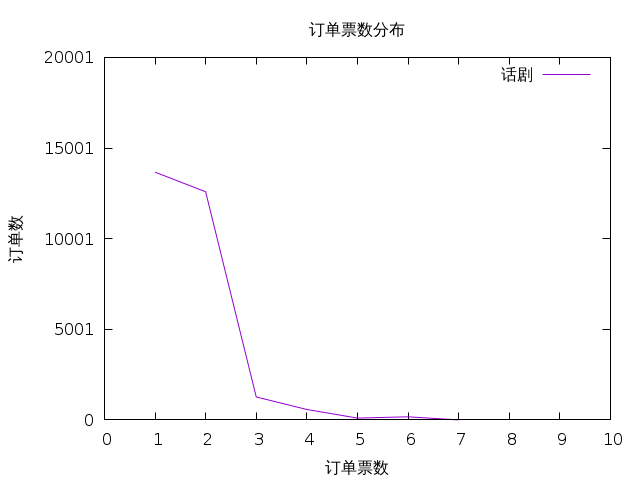
\includegraphics[width=.9\linewidth]{./image/drama-tickets-distribution.png}
\end{center}
\end{frame}

\begin{frame}[label={sec:org4659708}]{行为路径分析}
\alert{没做出来,未完待续\ldots{}}
\end{frame}
\begin{frame}[label={sec:org1619071}]{购买用户分析}
\begin{itemize}
\item 话剧类购买用户共 12441 人
\item 3781 个话剧购买用户会买其他类目
\item 5972 个话剧购买用户有复购行为
\end{itemize}
\begin{center}
\begin{tabular}{rr}
购买单数 & 用户数\\
\hline
1 & 12441\\
2 & 2981\\
3 & 1165\\
4 & 559\\
5 & 324\\
6 & 205\\
7 & 136\\
8 & 96\\
9 & 80\\
10 & 62\\
\end{tabular}
\end{center}
\end{frame}

\section{部分结论}
\label{sec:orgf3b17fe}
\begin{frame}[allowframebreaks,label=]{整体现象}
\begin{itemize}
\item 60\%的订单量在开演前两周内完成
\item 演唱会/话剧 2 个月内销量提升, 展览 2 周内, 其他类目 1 周内
\item 整体平台正价票销量最多
\item 演唱会折扣在 0.5-2 之间销量都还可以
\item 话剧折扣在 0.95-1 之间的销量最好
\end{itemize}
\framebreak
\begin{itemize}
\item 注册当天就购买的订单占比 90\%以上, 第二天还不买基本就不会买了
\item 除了演唱会,其余票价在 100-200 之间的销量最好
\item 演唱会票价对销量的影响更小, 在 200-600 之间都不错
\item 大部分的购买是冲动型, 5-10 分钟以内就决策决定买
\item 决策时间越长, 支付比例越高
\end{itemize}
\end{frame}

\begin{frame}[label={sec:orgbe5dc14}]{app 的数据}
\begin{itemize}
\item 一半以上在列表页能看到想看的(会进行点击)
\item 首页的退出率 12\%, 首屏的项目/栏目的吸引度/新鲜度不够
\item app 的转化漏斗大约为 详情->30\%(选票) -> (下单)12.3\% -> (支付) 16\% -> (支付成功) 28\%
\end{itemize}
\end{frame}

\begin{frame}[label={sec:org2454e21}]{演唱会类交易场景}
最大场景: 热门明星
\begin{itemize}
\item 价值点: 1. 信息(什么时候开)  2. 靠谱的买到 3. 价格合理的买到
\end{itemize}

次级场景(热点): 音乐节 生活节 逢年过节演唱会

其他场景: 搜索/浏览其他演唱会
\end{frame}
\end{document}